% Virtual Environment for Individual-Based Modeling - Part II
%
% Advanced Project II - Jacobs University Bremen
% Supervisor: Dr. Stefan Kettemann
%
% Created on January 10, 2019
%
% Authors:
%   Ralph Florent <r.florent@jacobs-university.de>
%   Davi Tavares <davi.tavares@leibniz-zmt.de>
%   Agostino Merico <a.merico@jacobs-university.de>
%
% Main entry for the documentation

% ==============================================================================
% START: Preamble
% ==============================================================================
\documentclass{article}

\usepackage{amsmath}
\usepackage{amssymb}
\usepackage[title]{appendix}
\usepackage{array}
\usepackage[british,UKenglish,USenglish]{babel}
\usepackage[backend=biber,style=numeric,sorting=none]{biblatex}
\usepackage[utf8]{inputenc} % required to load before csquotes
\usepackage{csquotes}
\usepackage{dirtree}
\usepackage{dirtytalk}
\usepackage[dvipsnames]{xcolor}
\usepackage{graphicx}
\usepackage[inner=3cm,outer=3cm,top=3cm,bottom=3cm]{geometry}
\usepackage{hyperref}
\usepackage{minted}
\usepackage{subcaption}
\usepackage{url}

% Override line interspace default configurations
\renewcommand{\baselinestretch}{1.5}

% Override Table default configurations
\setlength{\tabcolsep}{18pt}
\renewcommand{\arraystretch}{1.5}

% Override hyper reference default configurations
\hypersetup{
    colorlinks = true,
    linkcolor = blue,
    anchorcolor = blue,
    citecolor = blue,
    filecolor = blue,
    urlcolor = blue
}
\urlstyle{same}

\addbibresource{references.bib} % Input references by file
\graphicspath{{images/}} % Set path for image preloading

% set default color and style sheets for the scripts
\definecolor{bg-mint}{rgb}{0.95,0.95,0.95}

\title{
    {
\includegraphics[scale=0.15]{logo-black.png}} \\
    \vspace{1.2cm}
    {\large \textbf{ADVANCED PROJECT II}} \\
    {\large \textbf{Project Report}} \\
    {\large Supervisor: Prof. Dr. Agostino Merico} \\
    {\large Contributor: Dr. Davi Tavares} \\
    \vspace{1.2cm}
    {\large \textbf{Virtual Environment for Individual-Based Modeling - Part II}}
}

\vspace{1.2cm}
\author{ \textit{By Ralph Florent}}
\date{January 10, 2020}

% \vspace{1.4cm}
% ==============================================================================
% END: Preamble
% ==============================================================================

% ==============================================================================
% START: Scripts
% ==============================================================================
\begin{document}
\maketitle

% Abstract
% Individual-Based Modeling (IBM)
%
% Advanced Project I - Jacobs University Bremen
% Supervisor: Dr. Stefan Kettemann
%
% Created on May 29, 2019
%
% Authors:
%   Ralph Florent <r.florent@jacobs-university.de>
%   Davi Tavares <davi.tavares@leibniz-zmt.de>
%   Agostino Merico <a.merico@jacobs-university.de>
%
% Abstract block for the documentation

% ==============================================================================
% START: Abstract
% ==============================================================================

\begin{abstract}
This report provides some facilities for understanding the virtual environment implemented to study the habitat use by waterbirds in coastal lagoons of the tropics. This virtual environment is based on an Agent-Based Modeling system using some assumptions that are derived from previous observations of waterbirds' behavior within some habitats in the tropics. Further, some detailed information is given about the carried-out tests and their results.
\end{abstract}

% ==============================================================================
% END: Abstract
% ==============================================================================
\newpage

% Introduction
% Virtual Environment for Individual-Based Modeling - Part II
%
% Advanced Project II - Jacobs University Bremen
% Supervisor: Dr. Stefan Kettemann
%
% Created on January 10, 2019
%
% Authors:
%   Ralph Florent <r.florent@jacobs-university.de>
%   Davi Tavares <davi.tavares@leibniz-zmt.de>
%   Agostino Merico <a.merico@jacobs-university.de>

% ==============================================================================
% START: Introduction
% ==============================================================================

\section{Introduction}
The \emph{Virtual Environment for Individual-Based Modeling - Part II} is a continuation of the first release of the project whose purpose is to study the habitat use by waterbirds in coastal lagoons of the tropics while using the Agent-Based Modeling (ABM) techniques \cite{rflorent2019veibm1}. As mentioned in the outlook for the first version, we see space for additional features that will supposedly give a considerably fair understanding of the system, including its components. Hence, we have decided to implement new features to help conceive a dynamical system and simulate more physical characteristics of an interactive environment. But before going deep into more details concerning the newly-implemented features, namely their technical aspects, that are considered for the second release, let us first raise some relevant points about this project report.

\subsection{Assumptions}
Being the second part of the project defined to achieve a \emph{Virtual Environment (VE)} using ABM techniques to characterize the waterbirds behaviors, adaptation, and evolution within a set of habitats with distinguishable properties \cite{rflorent2019veibm1}, this report is indeed addressed to an audience with some practical understanding of the previous carried-out work\footnote{It is highly recommended to check out the documentation of the \emph{Virtual Environment for Individual-Based Modeling - Part I} project to grasp specific tightly-related concepts and understand certain decision-making when it comes to choosing between two(2) or more options. Refer to Appendix \ref{sec:code-repo} for more details on how to access this documentation.}. Additionally, it is expected that the reader possesses some knowledge on the following concepts: \emph{basic Python programming, descriptive statistics}.

Considering the statements mentioned above, it is assumed that the reader is already familiar with these concepts and therefore any mention of them will not be enforced through further detailed explanation in this document. However, although that broader explanation will not be provided throughout the following sections, particular notes and references will be intentionally used as a form of guidance for further readings.

\subsection{Motivation}
The idea of having a virtual environment for ABM systems is quite innovative. It attracts many social science disciplines and looks very promising from an end-user perspective. As for ecological systems, being able to replicate into the computing world a specific real-world environmental context or situation while considering all (or the major part) of its complexities and implications is an opportunity knocking for alliviating some research projects (accounting for bugdets, expenses, resources, etc.). This project itself is a good example to illustrate the importance of having a virtual environment for further analysis on ecological systems.

In addition to that, the realization of this project will provide the following benefits:
\begin{itemize}
    \item \textbf{Contribution to life science}: given that computational resources and equipment can be taken advantage of for heavy calculations, having the proper tools to carry out successfully related experiments is considered as an asset to the science community.
    \item \textbf{Contribution to waterbirds' lifestyle}: by simulating the waterbirds' life in a virtual environment, predictive analyses can help to determine factors that cause natural resources (food availabilty, drought) exhaustion or any other similar negative consequences, and take anticipated decisions to limit or mitigate them.
    \item \textbf{Intellectual Property}: not only the tool can contribute to a large community that supports advanced techniques to improve life science work, but the author of such a tool can also benefit from worldwide recognition and publications.
\end{itemize}

\subsection{General Comments}
Recalling that the following document is about the tool used to describe the interactions of the waterbirds within some habitats in the tropics, it is done in a very highly technical way. That is, since the key concepts of the virtual environment tool is explained in the first part of the project, the following sections dive deep down into the programming techniques used to implement it. With the purpose of providing an easy-to-follow guide to grasp the main idea behind the writing of this report, an overview of its structure is outlined below:
\begin{itemize}
    \item \textbf{Overview}: though it is not necessarily a concern, yet it is relevant to retake some of the notions discussed in the past work to facilitate the understanding of the terms that are used across the document. Parts of these notions are the basic theoretical background, the previous methods to operate the virtual environment, the obtained results and discussions, and the reasons for having a part two (2).
    \item \textbf{Features}: right after explaining the reasons of defining new goals and how to reach them, we discuss the new features considered for the VE. The most relevant features are the application of a dynamical environment (involving more environmental characteristics/properties), the increase of the number of species (waterbirds), the one-unit time processing implementation, and some techniques for further analyses.
    \item \textbf{Methodology}: Obviously, the procedural methods used in the past suffer some breaking changes while adding the new features and these changes are discussed in the corresponding section. Besides that, it is important to highlight certain points taken into account to ease up the development speed and productivity from a programmer's perspective.
    \item \textbf{Results}: the reported results vary as the environment changes. Hence, we expose and assess them while maintaining the scope closed and simple, and we provide some outlook given the impediments we have confronted.
\end{itemize}

Keep in mind that for each subtopic mentioned above, we break them down into smaller points to facilitate an easy-to-understand structure and elaborate supporting details. This report is also available on \href{https://github.com/}{GitHub} under a public repository: \href{https://github.com/systemsecologygroup/BirdsABM}{github.com/systemsecologygroup/BirdsABM}. Please refer to Appendix \ref{sec:code-repo} to know how to walk through the repository and contribute to this project in the future.
% ==============================================================================
% END: Introduction
% ==============================================================================

% Theory review
% Virtual Environment for Individual-Based Modeling - Part II
%
% Advanced Project II - Jacobs University Bremen
% Supervisor: Dr. Stefan Kettemann
%
% Created on January 10, 2019
%
% Authors:
%   Ralph Florent <r.florent@jacobs-university.de>
%   Davi Tavares <davi.tavares@leibniz-zmt.de>
%   Agostino Merico <a.merico@jacobs-university.de>

% ==============================================================================
% START: Overview of VE-IBM Part I
% ==============================================================================

\section{Overview}\label{sec:overview}
The goal of the first part of the \emph{Virtual Environment for Individual-Based Modeling} project was clear and simple: create a virtual environment prototype while using an ABM technique to study the habitat use by waterbirds in coastal lagoons of the tropics. Therefore, we built our assumptions on the general model concept shown below in Figure \ref{fig:concept-1v}.

As the second part of the project is built upon this first part, we retake some points that are relatively important and constitute the core element of the second release. In the section, we give an overview of the past work and discuss the correlation between both the first and second version.

\begin{figure}[!ht]
    \centering
    \frame{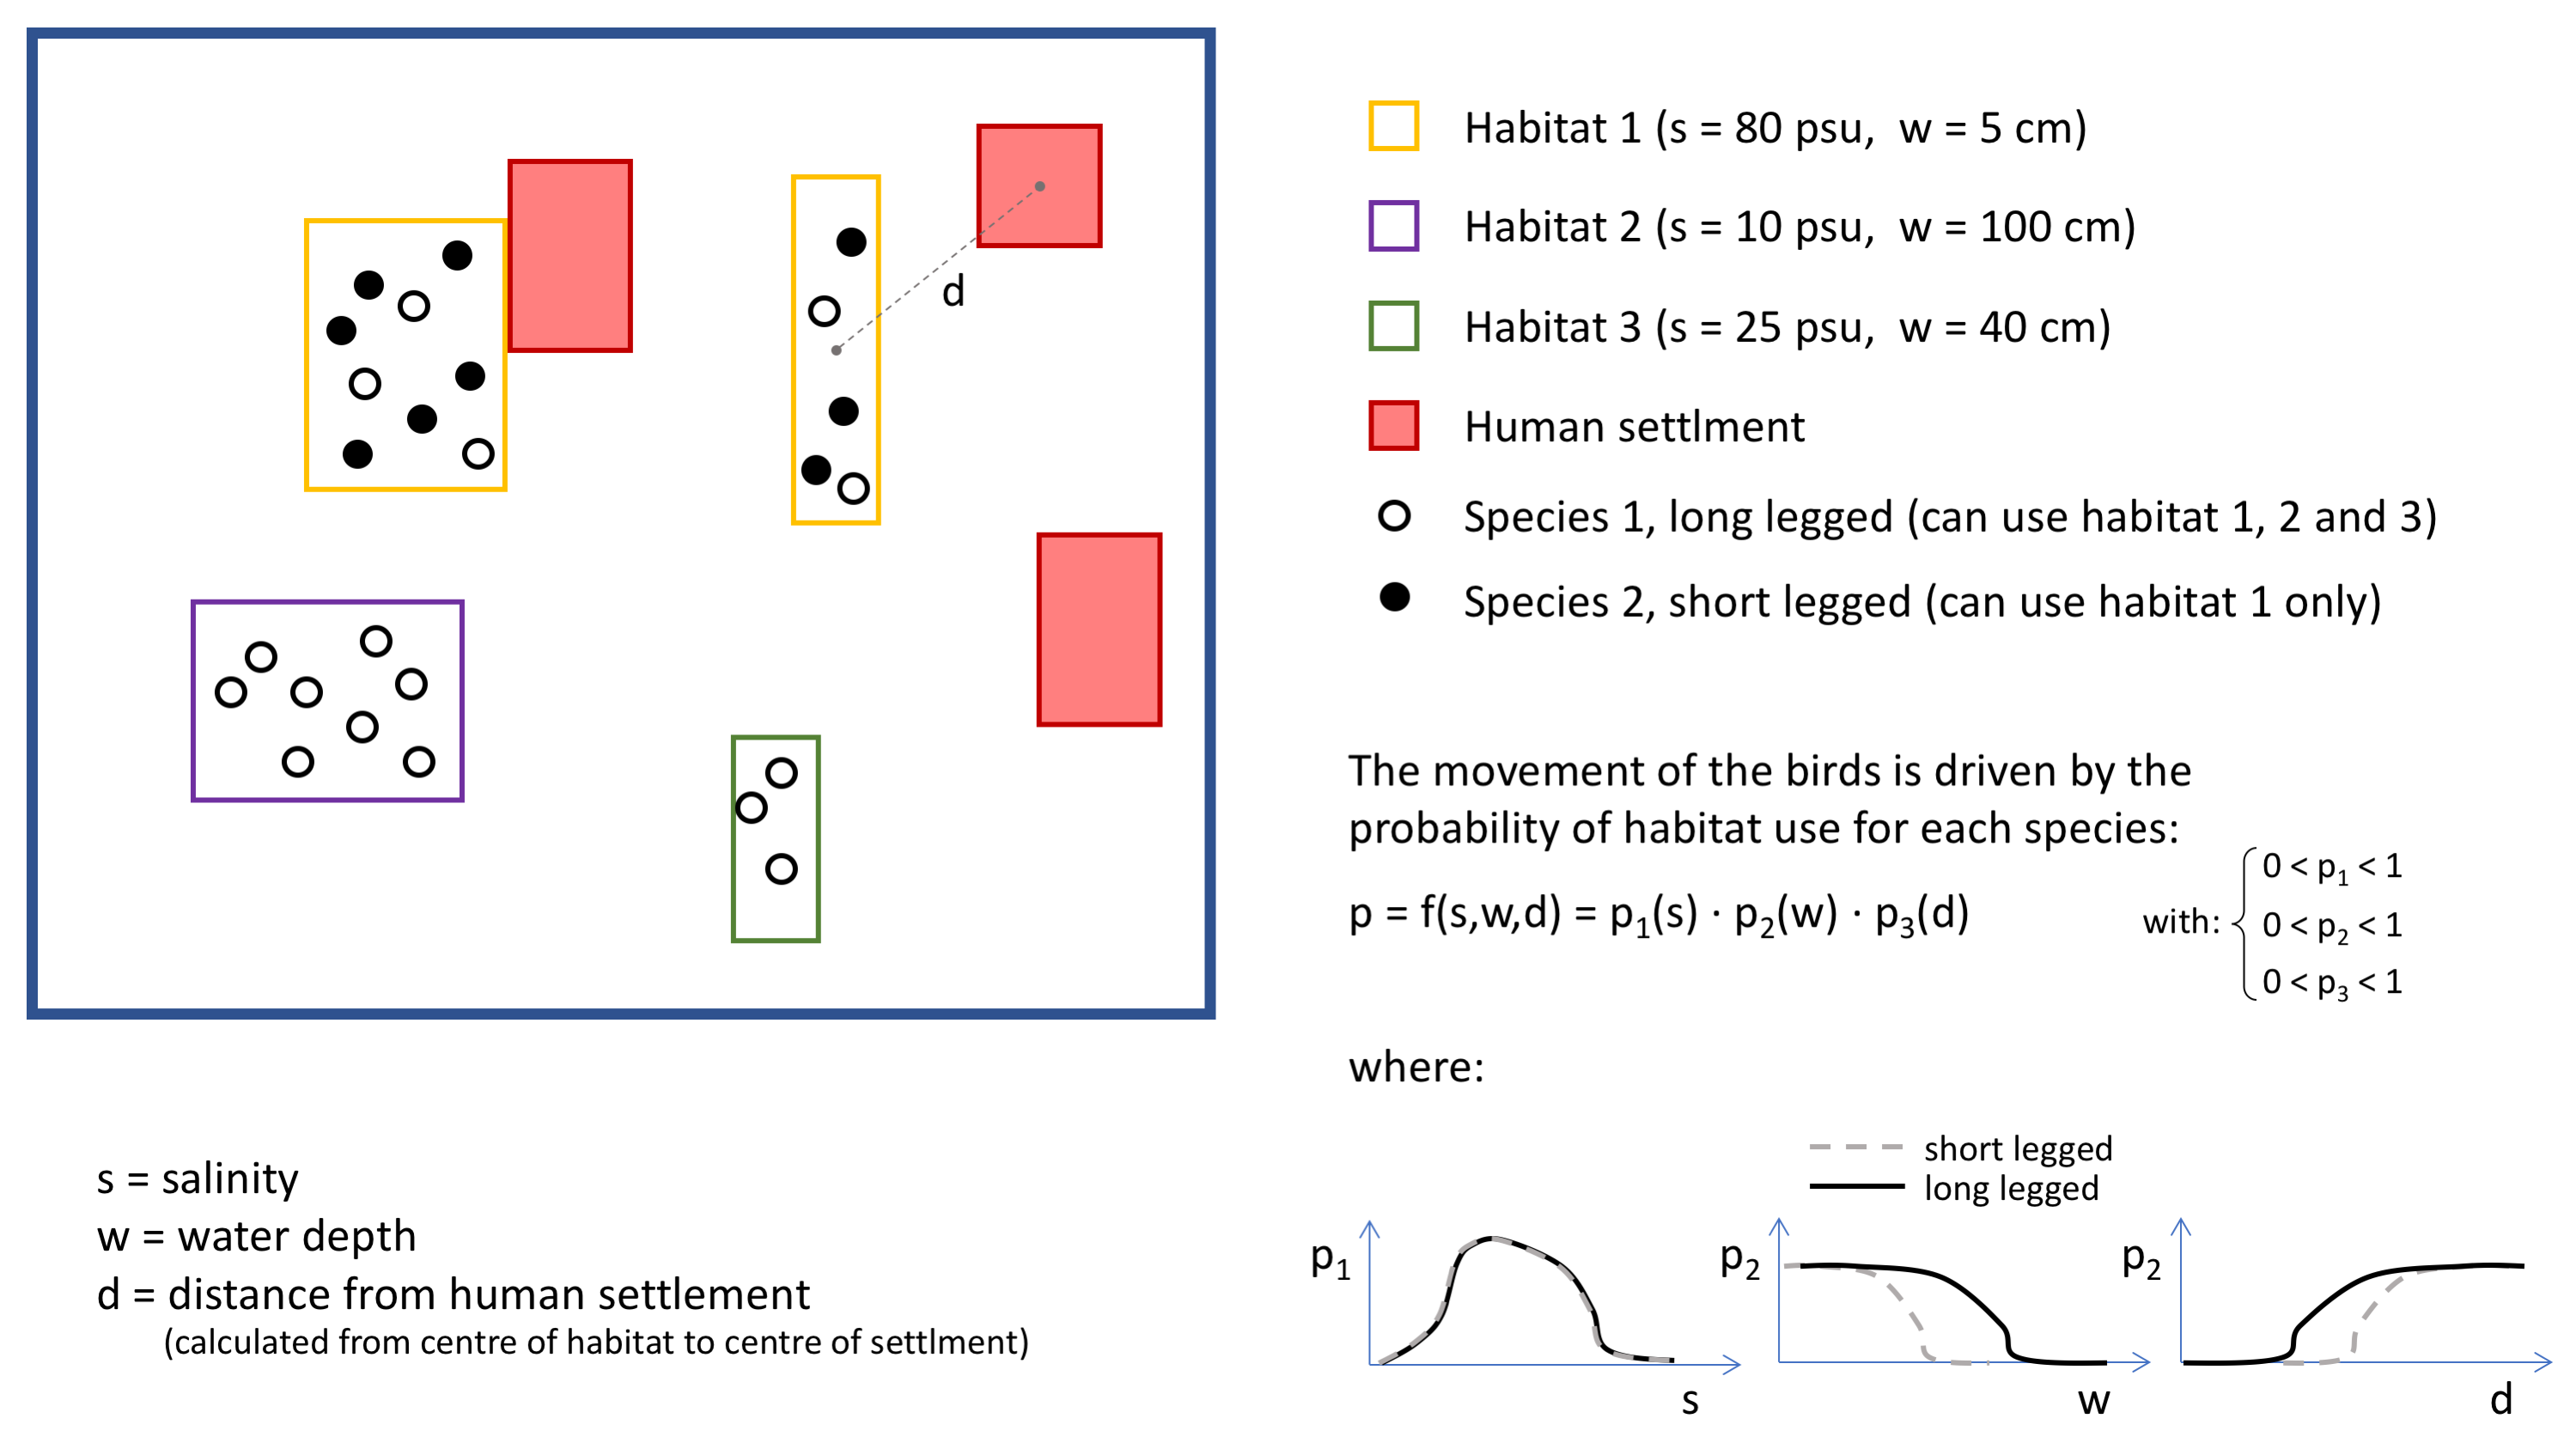
\includegraphics[scale=0.33]{docs/concept_1v.png}}
    \caption{Model concept for the \emph{Virtual Environment for Indivual-Based Modeling - Part I}.}
    \label{fig:concept-1v}
\end{figure}

\subsection{Theory review}
In the first part of the project, some core elements or components such as  \emph{warterbirds} and \emph{lagoons} of the system are discussed and, subsequently, their digital representation within the prototype based on the assumptions derived from previous investigations.

Recalling that tropical coastal lagoons are shallow aquatic ecosystems located at the boundary between terrestrial and marine environments \cite{tavares2015environmental}, the high environmental heterogeneity of coastal lagoons, in both temporal and spatial scales, provides habitats for aquatic bird species with different ecological needs \cite{ntiamoa1998water, paracuellos2004factors, tavares2013inventory}. Seven environmental variables mainly characterize these habitats and water depth is the most important variable influencing the waterbird assemblage \cite{tavares2015environmental}.

On the other hand, the aquatic birds or \emph{waterbirds} inhabiting the coastal lagoons were, according to a survey conducted by Tavares D.C. et al. in 2015 \cite{tavares2015environmental}, grouped into guilds\footnote{ Blondel proposed the guild concept in 2003 \cite{blondel2003guilds}.} reflecting species' foraging habits and morphology. The six identified guilds were: diving birds (grebes), dabbling ducks (belonging to the genera Dendrocygna and Anas), large wading birds (herons, egrets, and storks), vegetation gleaners (jacanas and gallinules), fishing birds (gulls and terns) and small wading birds \cite{tavares2014variaccao}.

Agent-Based Modeling is a computational simulation framework based on intense processing and algorithmic calculations due to the fact the typical context in which the ABM is used is to study the collective behavior of a large number of components or agents \cite{rflorent2019veibm1}.

\subsection{Methods}
The core functionality of the project is based on a programmatically-implemented coding procedure that allows to explore certain programming techniques and choose the most convenient workflow for building the first VE prototype.

Its workflow scheme (as illustrated in Figure \ref{fig:workflow-scheme}), includes some internal processes that were based on the following premises: \emph{Initialize, Observe}, and \emph{Update}, where:
\begin{enumerate}
    \item \textit{Initialize}: stands for initial conditions of the system
    \item \textit{Observe}: displays a snaphot of the current state of the system
    \item \textit{Update}: generates a new state of the system by computing some random movements of the agents (based on specific factors).
\end{enumerate}

\begin{figure}[!ht]
    \centering
    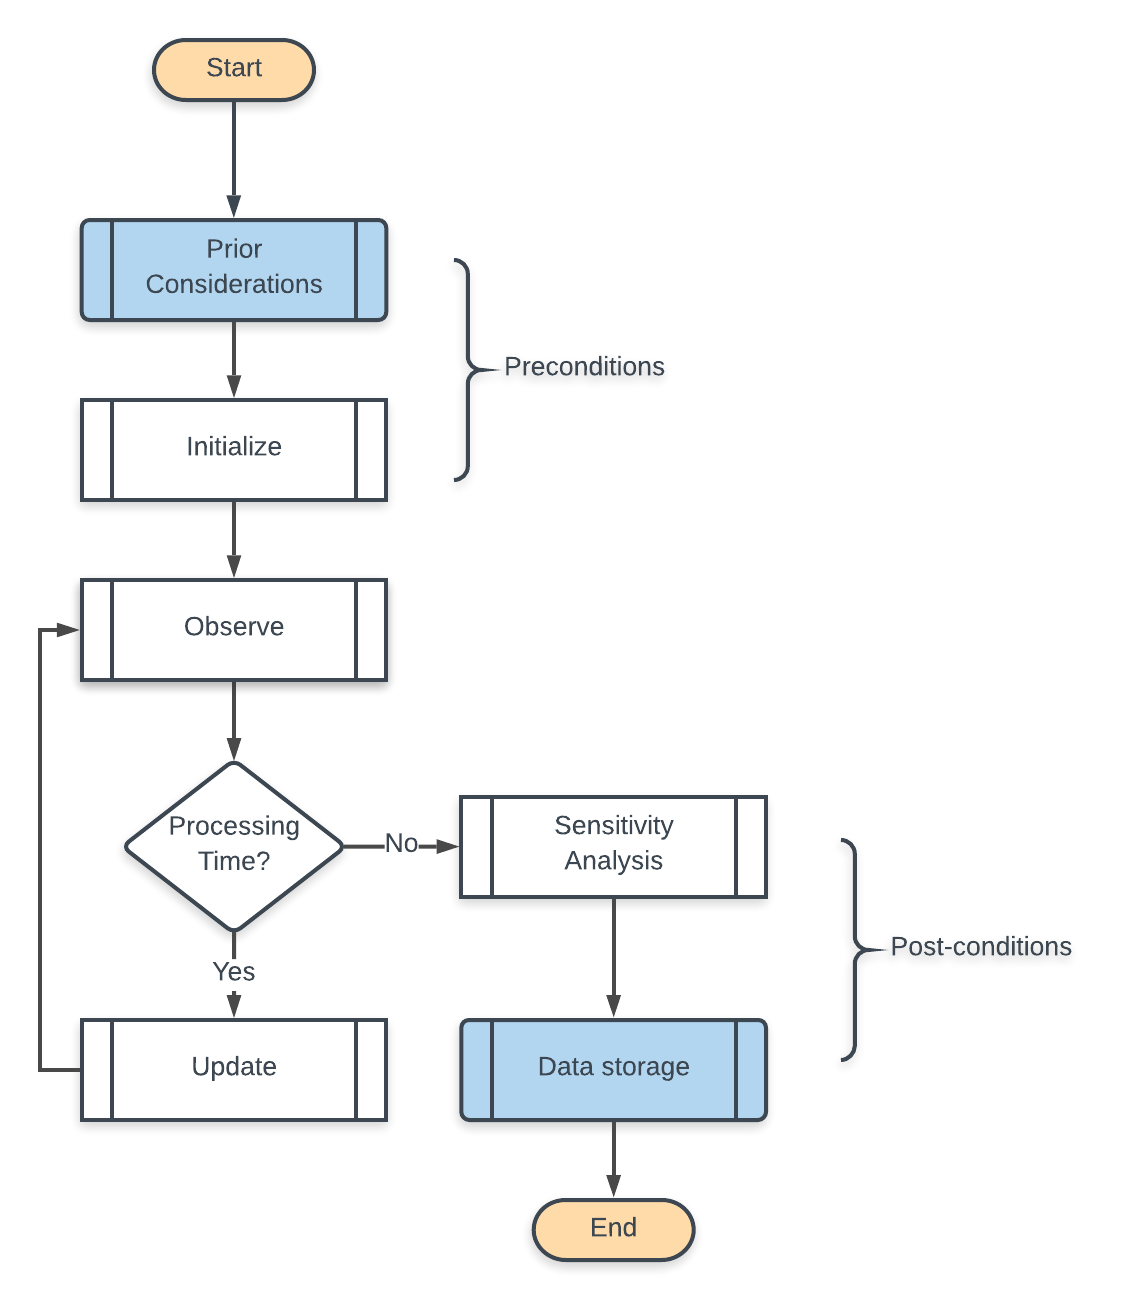
\includegraphics[scale=0.33]{docs/workflow-scheme.png}
    \caption{Workflow diagram \\ (credits: made with \emph{Lucidchart})}
    \label{fig:workflow-scheme}
\end{figure}

The VE prototype was essentially a digital representation of an ABM system where each component of that system relies on the interaction and interconnection with other involved elements in an organized flow. The diagram in Figure \ref{fig:workflow-scheme} was used as a visual aid expressing the intended performing flow of the components within the system.

\subsection{Results}
After conducting successfully two (2) pilot tests, we combined them to shape a final prototype that represents the model concept illustrated in Figure \ref{fig:concept-1v}.

Although this version of the VE simulation only considers certain factors that would interpret much closer to the waterbirds' lifestyle inhabiting the coastal lagoons of the tropics, yet the results were fairly satisfying. Let us retake some key notions (terms and concepts) used to ease up the interpretations of those results.
\begin{itemize}
    \item \textbf{Habitat}: a patch-focused drawing representation of the lagoons, rectangularly shaped and based on additional design settings.
    \item \textbf{Agent}: categorized as \emph{short-legged} or \emph{long-legged}, a drawing representation of the waterbirds.
\end{itemize}

It should be recalled that each run of the main script (available in Appendix \ref{sec:code-repo}) would generate different results since we did not handle a seed-oriented initial state (see Table \ref{table:ve-init}) for the components.

\begin{table}[!ht]
    \begin{center}
        \begin{tabular}{ ||l|l|| }
            \hline
            \multicolumn{2}{ ||c|| }{ \textbf{Initial Conditions}} \\
            \hline \hline % Table body (row-wise contents)
            \textbf{\textit{Total of long-legged waterbirds}} &  20 \\
            \hline
            \textbf{\textit{Total of short-legged waterbirds}} &  20 \\
            \hline
            \textbf{\textit{Processing times}} &  100 \\
            \hline
            \textbf{\textit{Threshold for }} &  $1 * e^{-7}$ \\
            \hline
            \textbf{\textit{Areas for short-legged waterbirds}} &  \texttt{one} \\
            \hline
            \textbf{\textit{Areas for long-legged waterbirds}} &  \texttt{one, two, three} \\
            \hline
            \textbf{\textit{Habitat one (big)}} & s = 80psu, w = 5cm, f = 0.3  \\
            \hline
            \textbf{\textit{Habitat one (small)}} & s = 80psu, w = 5cm, f = 2.56  \\
            \hline
            \textbf{\textit{Habitat two}} & s = 10psu, w = 5cm, f = 6.41  \\
            \hline
            \textbf{\textit{Habitat three}} & s = 25psu, w = 40cm, f = 11.53  \\
            \hline
        \end{tabular}
        \caption{Default values and parameters for the VE prototype's initial conditions.}
        \label{table:ve-init}
    \end{center}
\end{table}

As we do not intend to describe every detail of the results here, please refer the documentation of the first version (see Appendix \ref{sec:code-repo}) for further explanation.

\subsection{Outlook}
Note that in our previous work running the script would only generate a single-point dataset for each PDF over time. That is because at that time we did not consider a one-unit time processing where an \emph{update} action would be performed on every agent. Meanwhile, we discussed in the analysis of the results how to achieve a data set by tuning the habitats' characteristics and other influent factors over time. For instance, simulating a water depth reduction by including rainfall influence or tweaking the food availability factors are an excellent example of how to achieve a multi-point dataset for each PDF.

In addition to that, all the operations were executed in memory (CPU + RAM). No actual file dumping was being done. That was an exhausting condition for expensive computations and could even turn into memory leaks, among other consequences.

% ==============================================================================
% END: Overview of VE-IBM Part I
% ==============================================================================

% Contents
% Individual-Based Modeling (IBM)
%
% Advanced Project I - Jacobs University Bremen
% Supervisor: Dr. Stefan Kettemann
%
% Created on May 29, 2019
%
% Authors:
%   Ralph Florent <r.florent@jacobs-university.de>
%   Davi Tavares <davi.tavares@leibniz-zmt.de>
%   Agostino Merico <a.merico@jacobs-university.de>
%
% 1) Introduction
% 2) Theoretical background
% 3) Instrumentation (software and tools)
% 4) Methods (Procedure)
% 5) Results, Discussions
% 6) Conclusion
% 7) References

% ==============================================================================
% START: Methods, Results, Discussions, Conclusion
% ==============================================================================

\section{Instrumentation}
The VE, as specified literally, is developed in a complete \emph{virtualized} workspace. This virtualized workspace is made up of tools and software used to carry out this project to its current release. In this section, a brief overview of those tools and software is provided to help to reproduce or replicate the exact setup of the development environment put in place at the time of implementing the project.

\subsection{Tools and Software}
Several currently-available programming tools may achieve the same VE goal. The reason to believe so is that it turns out that today's open source community has grown larger and, subsequently, has been more actively involved in software improvements and new releases. As a result, accessing those online tools is no longer an issue, at least in terms of low-money budget, since they are publicly available (under free or moderately limited license).

Given the availability of several options, enlisted below are the most natural choices of  tools and software for a developer with mere knowledge in programming:
\begin{itemize}
    \item GNU/Linux Ubuntu 16.04 (operating system)
    \item Visual Studio Code (text editor for the documentation)
    \item Git\footnote{Also available as a bash emulation for other platforms for free (e.g., Git Bash for Windows).} (version control)
    \item GitHub (web-based hosting service for versioning system)
    \item Python (programming language for the scripting)
    \item Jupyter Notebook (workspace for the VE simulation)
\end{itemize}

\noindent
It is not a concern to access and use a set of randomly compatible versions of the tools and software mentioned above. However, in case a developer wants the exact versions, Table \ref{table:tools-and-software} lists more detailed information on both the releases and sources for future downloads.

\begin{table}[!ht]
    \begin{center}
        \begin{tabular}{ |l|l|l|l| }
            \hline
            \multicolumn{4}{ |c| }{ \textbf{Tools \& Software}} \\
            \hline % Table headers
             & \textbf{Versions} & \textbf{Sources} & \textbf{Cost}  \\ [0.5ex]
            \hline % Table body (row-wise contents)
            \textbf{\textit{Visual Studio Code}} & 1.34.0 & See \cite{vscode} & Free  \\
            \hline
            \textbf{\textit{Git}} & 2.7.4 & Built-in Linux program & Free  \\
            \hline
            \textbf{\textit{GitHub}} & N/A & See \cite{github} & 5 free users  \\
            \hline
            \textbf{\textit{Python}} & 3.5 & See \cite{python} & Free  \\
            \hline
            \textbf{\textit{Jupyter Notebook}} & 5.7.4 & See \cite{jupyternotebook} & Free  \\
            \hline
        \end{tabular}
        \caption{Detailed information on the tools and software used for the VE}
        \label{table:tools-and-software}
    \end{center}
\end{table}

\subsection{General Comments}
The tools and software discussed in the previous subsection are chosen by a matter of personal preference. No further comparison or parallelism procedure has been carried out to assess the most convenient option. That is to say, it might exist a better work environment where the VE simulation is simpler and/or easier, or the VE surprisingly performs better\footnote{In the outlook section, "simpler" and "easier" simulation is explained with the perspective of an ideal use case scenario. Similarly, improved performance of the VE refers to a reduction in processing time, resource consumption in an easy-to-follow simulation platform.}. But, given that this first release is most importantly seen as a prototype, more tools and software can be tested out in a near future so that we end up with a so-called optimal workspace for the VE.

\section{Methodology}
This section will explore the methods used to implement the core functionality of this project. This exploration includes the mention of the workflow scheme, the third-party libraries usage and options, the algorithm and content structure, and finally, the programmatically-implemented coding procedure.

\subsection{Workflow Scheme}
This project's workflow scheme consists of 3 main steps:
\begin{enumerate}
    \item \textit{Initialize}: stands for initial conditions
    \item \textit{Observe}: handles the graphical parts
    \item \textit{Update}: computes random movements based on the probability distribution of the corresponding factors.
\end{enumerate}
where each step contains itself a series of internal subprocesses aiming a specific goal.

\begin{figure}[h!]
    \centering
    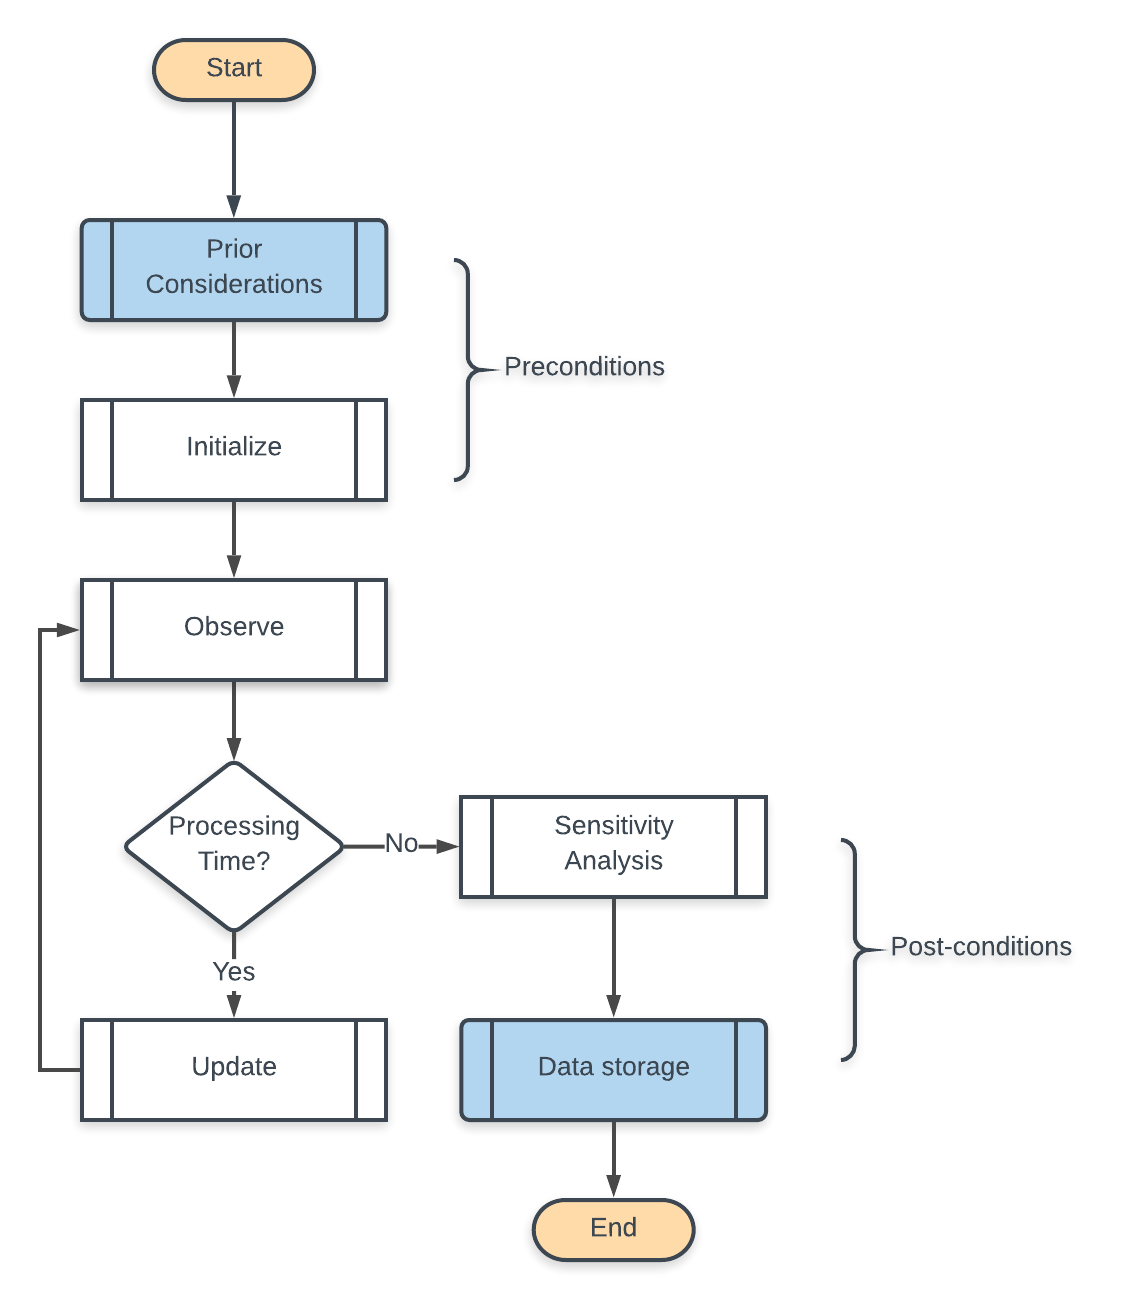
\includegraphics[scale=0.33]{docs/workflow-scheme.png}
    \caption{Workflow diagram \\ (credits: made with \emph{Lucidchart})}
    \label{fig:workflow-scheme}
\end{figure}

\noindent
\textbf{Important}: \textit{Observe in Figure \ref{fig:workflow-scheme} the remaining steps categorized as \emph{Preconditions} and \emph{Postconditions}. They represent respectively the \emph{Before} and \emph{After} the 3 main steps \texttt{Initialize, Observe}, and \texttt{Update} are executed. Note also that the \texttt{Initialize} process is considered part of the Preconditions semantics. That is because it only prepares the basic conditions for the components of the system, which are the habitats and the birds.}

Analyzing the workflow diagram in Figure \ref{fig:workflow-scheme}, we denote the following fields:
\begin{itemize}
    \item \textbf{\textit{Start}}: indicates the starting point of the VE simulation.
    \item \textbf{\textit{Prior Considerations}}: are the basic setup necessary to fulfill the initialization phase requirements\footnote{These considerations, mostly based on the concerned entities (waterbirds, coastal lagoons), the environmental variables, and any additional properties contributing to the setup phase of the VE simulation, are also discussed in this document in the theoretical section.}. This setup spans the following elements: the geometry of the habitats and the human settlements; the functions defining the probability distribution of the random movements (driven by the water salinity, water depth, and food availability factors); the duration of the overall simulation process; and a reasonable threshold to handle the feasibility of the random movements for a given seabird under certain conditions.
    \item \textbf{\textit{Initialize}}: creates the initial conditions of the system based on prior considerations mentioned above. That is the patches (habitats) and agents (seabirds) creation.
    \item \textbf{\textit{Observe}}: generates a 2-dimensional plot whose scale goes from zero to one(\emph{$0-1$}) in both axes (x, y). The rendered plot helps to visualize both the patches' and agents' positions.
    \item \textbf{\textit{Processing Time?}}: focuses on updating the agents' positions' as long as the conditional parameter for the processing time holds. That is, the iteration is exclusively based on a specific number of times without accounting for other parameters that might influence the habitats and the birds. Note that, in this current version, the iteration is set statically during the prior considerations process.
    \item \textbf{\textit{Update}}: randomly assigns an agent to new positions within the existing habitats, considering a given threshold and the other aspects of the probability distribution.
    \item \textbf{\textit{Sensitivity Analysis}}: collects the probability values to form a set of probability distributions, which later can be analyzed and compared to each other with the expectation to draw conclusions on the final output.
    \item \textbf{\textit{Data Storage}}: given the generated plots, collects them as PNG images, and then generates a GIF out of the entire dumped images. That is relevant to provide the end-user useful insights on the collected data.
    \item \textbf{\textit{End}}: indicates the ending point of the VE simulation.
\end{itemize}

Recalling that this Virtual Environment constitutes essentially a digital representation of an Agent-Based Modeling system, each component of such a system relies on the interaction and interconnection with other involved elements in an organized flow. Therefore, the diagram in Figure \ref{fig:workflow-scheme} shows a workflow scheme that intends to provide a visual aid for a better understanding of the system's behavior.

\subsection{Algorithm \& Data Structure}
The VE simulation implies the use of well-coordinated processes and subprocesses, which, once computed, will eventually attempt to explain the agents' behavior and their mutual interactions with the environment in which they coexist. This section discusses the algorithm and data structure applied to construct these processes and subprocesses.

\subsubsection{The \emph{Habitat} and \emph{Agent} data structure}
In the VE simulation, both the wetland areas and the human settlements of the coastal lagoons are represented by the term \emph{Habitat}\footnote{Note that human settlements are less appealing habitats for the waterbirds due to the humans' threatening characteristics}, and the waterbirds, by the term \emph{Agent}. In this case, the concept "Habitat"  is a 2-dimensional \emph{static} polygonal shape drawn from certain given geometrical measurements (see Figure \ref{fig:data-structure}). Similarly, the concept "Agent" is simply the representation of the waterbirds with some of its characteristics or attributes.

\begin{figure}[h!]
    \centering
    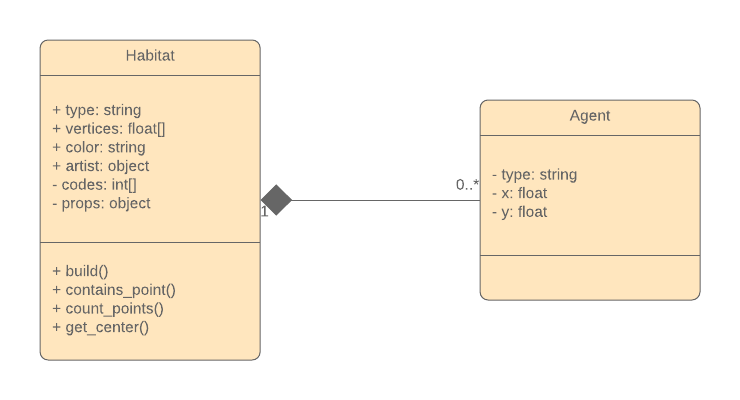
\includegraphics[scale=0.33]{docs/data-structure.png}
    \caption{Data structure of \emph{Habitat} and \emph{Agent} \\ (credits: made with \emph{Lucidchart})}
    \label{fig:data-structure}
\end{figure}

\noindent
Observe that in Figure \ref{fig:data-structure}, we use the class diagram named \emph{UML (Unified Modeling Language)} to model and document the properties of the components: Habitat and Agent. On the one hand, we construct a \textcolor{orange}{Habitat} class definition with the following properties:
\begin{itemize}
    \item \textbf{\textit{type}}: the type or category name of the habitat;
    \item \textbf{\textit{vertices}}: the coordinates of the patch representing the habitat;
    \item \textbf{\textit{color}}: the color (edge and face) to apply or distinguish a habitat from another;
    \item \textbf{\textit{artist}}: the patch-based polygonal shape to draw on a given figure;
    \item \textbf{\textit{props}}: the dictionary-like additional properties that characterize this habitat;
    \item \textbf{\textit{build()}}: constructs the \emph{artist} or patch on a figure;
    \item \textbf{\textit{contains\_point()}}: determines whether or not an x-y coordinate (point) belongs to a patch;
    \item \textbf{\textit{count\_points()}}: counts the total number of agents located within the patch based on their x-y positions.
    \item \textbf{\textit{get\_center()}}: obtains the center point (x-y coordinate)  of this habitat.
\end{itemize}

\noindent
On the other hand, we construct an \textcolor{orange}{Agent} class definition with the following properties:
\begin{itemize}
    \item \textbf{\textit{type}}: the type or category name of the agent species;
    \item \textbf{\textit{x}}: the x-coordinate of the agent within an area;
    \item \textbf{\textit{y}}: the y-coordinate of the agent within an area.
\end{itemize}

\noindent
\textbf{Important}: \textit{Keep in mind that some of the methods in the class definitions use helper functions to do their specific task. These helpers can be found in the Python scripts located in Appendix \ref{sec:code-repo}.}

\subsubsection{The overall algorithm}
The overall algorithm is quite based on the step-by-step flow chart described in Figure \ref{fig:workflow-scheme}. In other words, it corresponds to the descriptive, logical aspects of the core functionality of the VE. The steps are as follows:

\begin{enumerate}
    \item \textbf{\textit{Given}}: given a collection of geometrical measurements (design) of the existing habitats and human settlements in a specific environment, a finite number (relatively small, 20 for example) of seabirds, and a set of predefined probability distribution functions (PDF) whose arguments are the characteristics of that environment;
    \item \textbf{\textit{Initialization}}: represent digitally (virtually) that environment by creating patches and agents;
    \item \textbf{\textit{Update}}: randomly choose an agent, then assess the probability of it moving to a random destination, and finally move the agent (if doable);
    \item \textbf{\textit{Observe}}: snapshot the current state of the plotted environment, then save figure as a PNG image;
    \item \textbf{\textit{Iterate}}: Repeat steps \textbf{3} \& \textbf{4} for $n$ times;
    \item \textbf{\textit{Stop}}: collect the dumped images and form GIF final image to visualize the random movements of the agents.
\end{enumerate}

\subsubsection{The \emph{Update} algorithm}
Some of the processes are straightforward and do not demand a time-, or energy-consuming logic to build them. For instance, the initialization phase is one of the common cases where the developer only needs to take care of statically sets of values required as prior considerations for the initial conditions. But, as for the \emph{Update} process, a rational, analytical solution is needed.

This algorithm defines an asynchronous approach to update an agent's status, namely its geolocation randomly. Thus, the set of instructions that follows below is the algorithm used to accomplish the "\emph{Synchronous Update}" functionality of the VE simulation:

\begin{enumerate}
    \item \textbf{\textit{Given}}: given a randomly selected agent;
    \item \textbf{\textit{Initialization}}: randomly choose a new destination within an "acceptable" habitat (an area where this agent can move to, given the environmental conditions);
    \item \textbf{\textit{Computation}}: compute the probability of that new destination use for this agent.
    \item \textbf{\textit{Update}}: finally, move the selected agent to that new destination if the calculated probability complies with the threshold.
\end{enumerate}

Recalling that this version of the project is a prototype whose purpose is to virtualize a static Agent-Based Modeling system, these algorithms are defined in their most simplistic model. For this reason, they are subject to change in the future when it comes to updating the dynamics of the system or adding more complex variations.

\subsection{Implementation}
As mentioned in the \emph{Tools and Software} subsection in \emph{Instrumentation}, the VE simulation is implemented in a Jupyter Notebook workspace using the Python programming language. They are many reasons for choosing this particular setting to develop this workspace, and the free cost is one of them.

The code implementation is based on the flow diagram presented in Figure \ref{fig:workflow-scheme} as well as the algorithms and data structure described in the previous subsection. Here, we mostly focus on the coding procedure and the programming standards to facilitate other collaborators' contributions and support in the future.

A standard programming workflow, if it does not involve too much of team management, demands to follow a set of intended principles\footnote{Those principles vary among institutions. So far, there is not yet a clear proposed draft describing them. Therefore, supporting them remains subjective.} that takes a system from a development stage to a production stage. For instance, the code should be: \textit{architected, modular, standardized, structured, scalable, secure, performance-oriented, tested, testable, collaborative, time-estimated, documented, and so on}\cite{smashingmagazine}. These principles are prevalent among big tech companies' projects and can also be used for smaller, or startup projects.

Since this original version of the VE simulation is an early prototype, we focus on following part of these principles so far. Among them, figure:
\begin{itemize}
    \item \textbf{\textit{architected}}: the overall system follows a series of well-planned, modularized, interconnected conceptual tasks describing the interaction of the components within the system;
    \item \textbf{\textit{standardized}}: the script follows the rules for the naming conventions in Python (variable names, function and class definition, etc);
    \item \textbf{\textit{structured}}: the script is written semantically and logically, and organized sequentially (3rd-party libraries import, constants declaration, functions definition, and \emph{main}\footnote{Main entry function to run an application});
    \item \textbf{\textit{scalable}}: the script can be easily extended for new releases and anticipates enhancements in the future;
    \item \textbf{\textit{collaborative}}: the code is version-controlled using Git and GitHub online hosting service;
    \item \textbf{\textit{documented}}: the script is well-documented and describes the coding content in a very human-friendly way.
\end{itemize}

Besides the coding procedure, we also created a commonly-standardized, organized file structure (See Figure \ref{fig:file-structure}) for the project. Note the parent folders named \textit{\textcolor{blue}{src}} and \textit{\textcolor{blue}{docs}}. The former is for the source code of the project and the latter, for the documentation. The contents under those folders are backed-up and synced with an online GitHub repository for versioning and collaboration reasons.

Writing test is currently out of the scope of this release. We understand that using \emph{Unit Testing} and \emph{Integration Testing} for the implemented code is relatively essential and should be covered. For now, the coding is maintained and tested throughout the outputs and the visualizations as expected. But as for future updates or releases, the new implementation should be written using test-driven scripts methodology as the scalability of the project will make the code cumbersome to maintain and test.

\begin{figure}[h!]
    \centering
    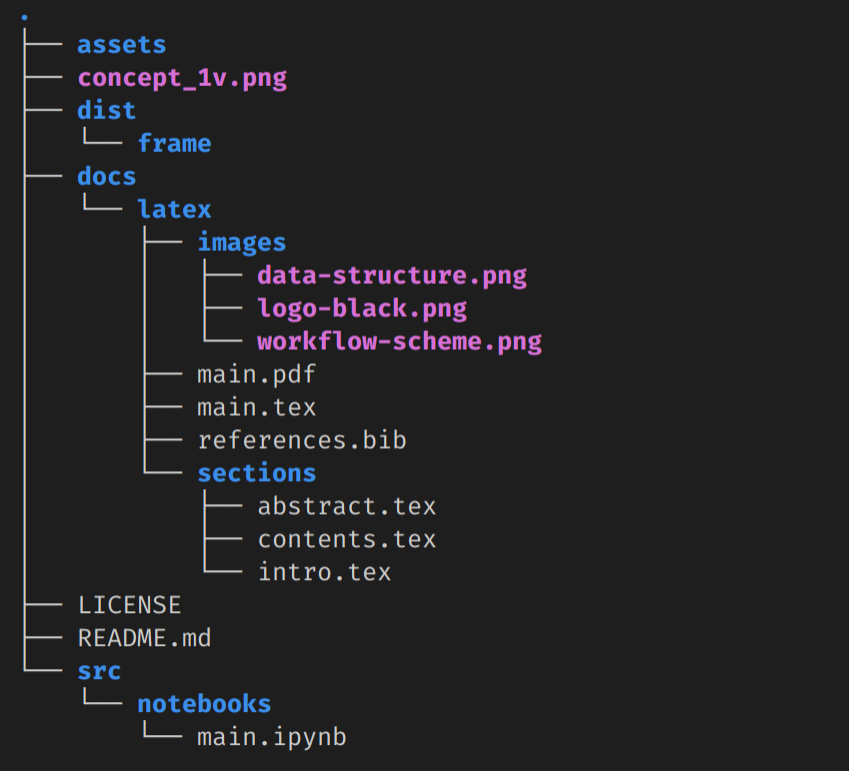
\includegraphics[scale=0.33]{docs/file-structure.png}
    \caption{File structure of the project}
    \label{fig:file-structure}
\end{figure}

\subsection{Third-Party Libraries}
Like in most of the software-based systems, not all the components (or parties) of such systems are built from scratch. That is also true for our VE simulation prototype. It is built on top of specific third-party libraries, as illustrated in Table \ref{table:third-party-libraries}.

\begin{table}[!ht]
    \begin{center}
        \begin{tabular}{ |l|l|l|l| }
            \hline
            \multicolumn{4}{ |c| }{ \textbf{Third-Party Libraries}} \\
            \hline % Table headers
             & \textbf{Versions} & \textbf{Sources} & \textbf{Features}  \\ [0.5ex]
            \hline % Table body (row-wise contents)
            \textbf{\textit{numpy}} & 1.15.4 & See \cite{numpy.random.rand,numpy.linalg.norm} & \textit{random, linalg.norm}  \\
            \hline
            \textbf{\textit{matplotlib}} & 3.0.2 & See \cite{matplotlib.patches,matplotlib.path,matplotlib.pyplot} & \textit{patches, path, pyplot}  \\
            \hline
            \textbf{\textit{imageio}} & 2.4.1 & See \cite{imageio} & \textit{imread, mimsave}  \\
            \hline
        \end{tabular}
        \caption{Detailed information on the third-party libraries used in the VE simulation}
        \label{table:third-party-libraries}
    \end{center}
\end{table}

One of the core principles in Software Engineering is \emph{DRY (\textbf{D}o not \textbf{R}epeat \textbf{Y}ourself)}. This acronym encourages developers to avoid code duplication and focus on configurable and reusable components \cite{scalablepath}. With that being said, we focus mainly on some third-party component reusability. That, of course, comes with its pros and cons:
\begin{itemize}
    \item \textbf{\textit{pros}}: time saving, pre-tested code usage, modular code usage, etc.
    \item \textbf{\textit{cons}}: dependency, lack of support, overuse, security issues, etc.
\end{itemize}

\noindent
The key point behind this brief pros-and-cons topic is to signal that it is crucial to carefully select the right libraries to use, which is what we did in the first place.

\section{Results \& Discussions}
The virtual environment prototype is the end-result of 2 combined pilot tests following the general model concept illustrated in Figure \ref{fig:concept-1v}. The results of these tests are presented in the subsections that follow.

\begin{figure}[h!]
    \centering
    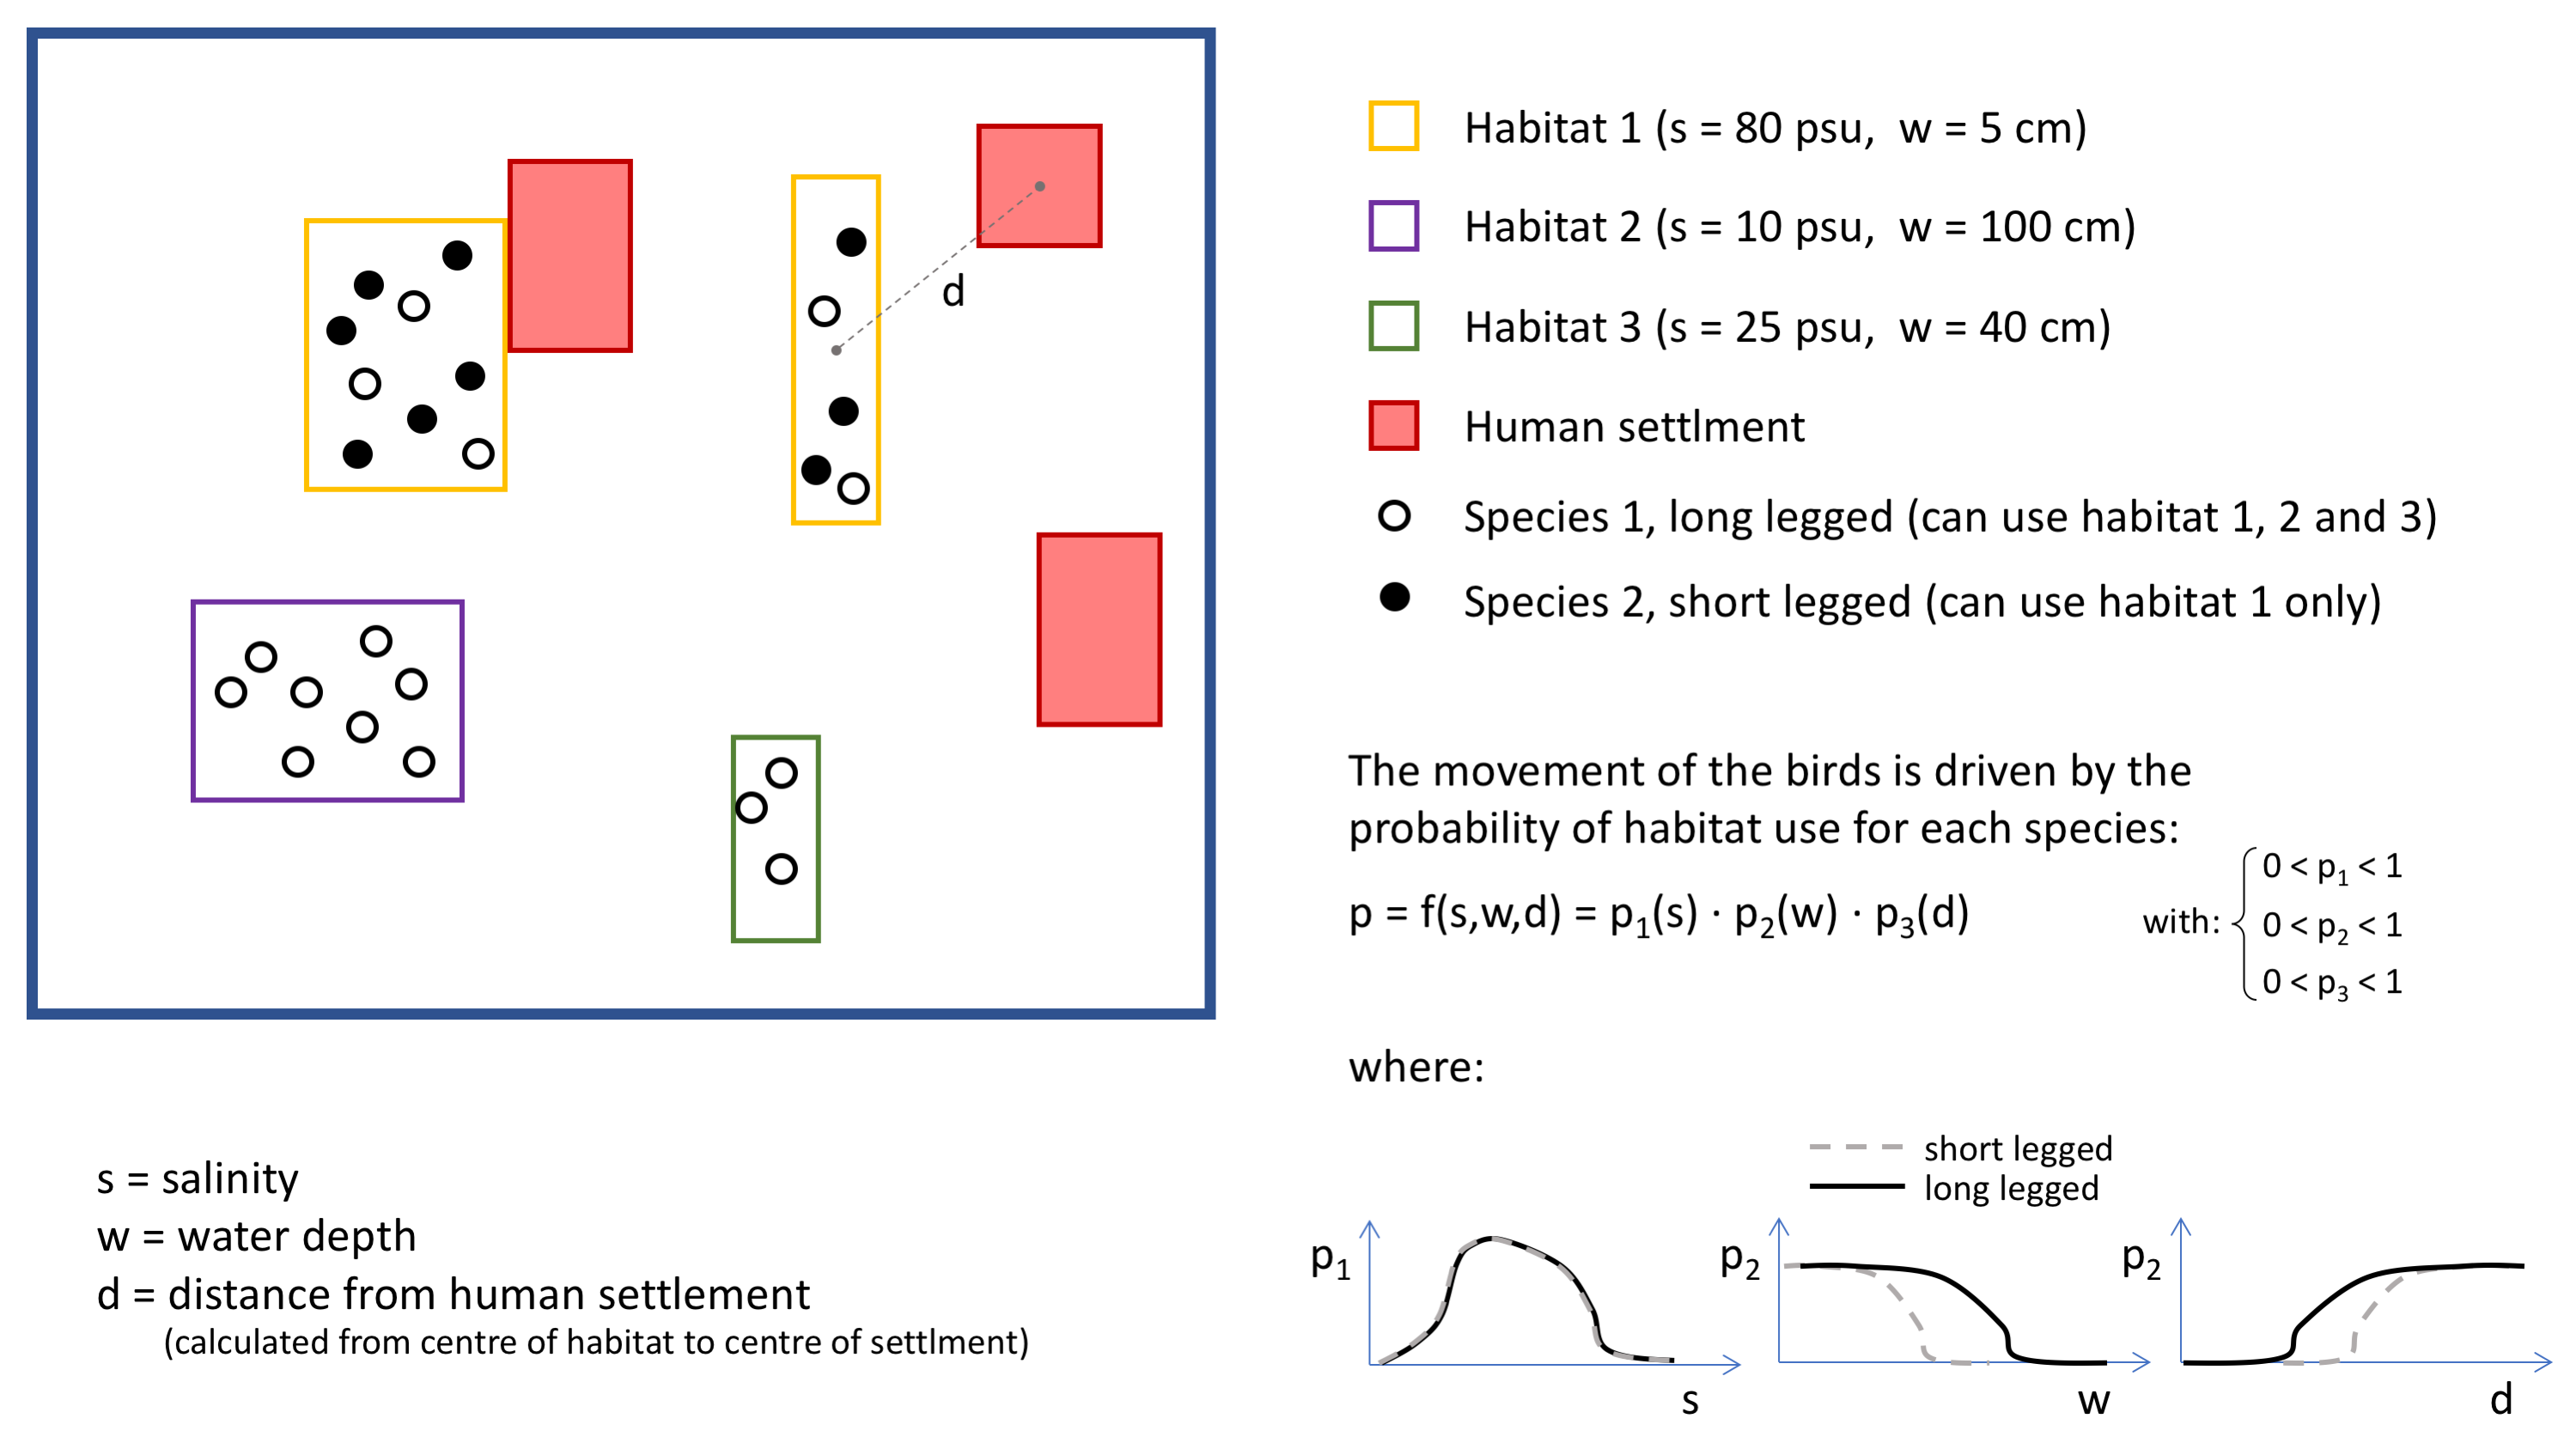
\includegraphics[scale=0.33]{docs/concept_1v.png}
    \caption{The general model concept for studying habitat use by waterbirds in coastal lagoons of the tropics. The functions for calculating the probability of birds moving using a given water depth, distance from human settlement and salinity can be found in Appendix \ref{sec:code-repo}.}
    \label{fig:concept-1v}
\end{figure}

\subsection{First Pilot Test}
In this very first test, we aim for the most possible, simplistic Agent-Based Modeling simulation. The objective of this test is to simulate a physical environment of static habitats and a few randomly-positioned waterbirds with the expectations of moving around over time. In addition to that, we create a simple restriction rule, which is "\textit{the waterbirds are not allowed to visit the habitats}".

Simulating this startup environment requires a focus on drawing specific patches (representing the habitats) and generating a finite number of agents (representing the waterbirds). In this case scenario, we use a square figure scaled from 0 to 1 in both sides as the limited area for the environment (see Figure \ref{fig:pilot-test-1}). Then, with the help of the \emph{matplotlib} 3rd-party library, we produce the patches. Similarly, we use object-based definitions to create the agents and randomly position them within the environment using some helper functions — no prior considerations.

\subsubsection{The patches}
A patch is a drawing version of a habitat. It has a non-, or polygonal shape and tries to represent as closely as possible a 2-dimensional structure in reality. The shape can be very simple, as in the case of a simple square; and very complex, as in the case of a curvy closed-line. Besides its structural representation, a patch has some other properties such as \emph{facecolor}, \emph{edgecolor}, \emph{lineweight}, and so forth, that are related to the setting of the drawing itself (see more details in \cite{matplotlib.patches}). But in our case, we choose to go with the rectangular shape, which we consider sufficient for the demo.

In earlier sections of this document, we introduced the \textcolor{orange}{Habitat} class definition with some attributes (\emph{type, vertices, color, etc.}) that is to represent a natural habitat or human settlement digitally. But in this first pilot test, we use only a lightweight version of these attributes, which are the vertices. To illustrate our point about drawing a patch (or an artist) within an area, see the Python scripts below:

\begin{listing}[H]
    \inputminted
    [
        baselinestretch=1.2, % interspace size
        bgcolor=darkgray,
        fontsize=\footnotesize,
        linenos % show line numbers
    ]
    {python}{scripts/intro-patch.py}
    \caption{Script for creating a patch using \emph{matploblib}}
    \label{lst:intro-patch}
\end{listing}

\noindent
Observe how the codes in lines 23-24 in Listing \ref{lst:intro-patch} create a final plottable object that can be later drawn in a figure.

\subsubsection{The agents}
An agent is a drawing version of a waterbird. It can be of the type \emph{short-legged} or \emph{long-legged} species. This little nuance is what constitutes the core distinction in the waterbirds' behaviour within the habitats. Therefore, it remains relevant to set a clear cut in the design so that a short-legged type visually differs from a long-legged type.

Recall that the \textcolor{orange}{Agent} class definition is really simple in terms of properties: \emph{type and x-y positions}. The \emph{type} attribute takes the value of either "short-legged" or "long-legged" and the agent's position is the $x$-$y$ coordinates that take decimal values between zero (0) and one (1) within a 2-dimensional area. As a result, creating an agent in the VE simulation is to instantiate an object of the on-the-fly class \textcolor{orange}{Agent}, then define its type as "short-legged" or "long-legged", and finally assign a random position to that agent. However, due to the restriction rule mentioned previously, the randomly-generated positions cannot fall into the area occupied by the habitats.

\begin{listing}[H]
    \inputminted
    [
        baselinestretch=1.2, % interspace size
        bgcolor=darkgray,
        fontsize=\footnotesize,
        linenos % show line numbers
    ]
    {python}{scripts/intro-agent.py}
    \caption{Script for creating an agent using the \emph{gen\_random\_point()} helper}
    \label{lst:intro-agent}
\end{listing}

Finally, the results of creating both patches and agents for the first pilot test are illustrated in Figure \ref{fig:pilot-test-1}.

\begin{figure}[h!]
    \centering
    \includegraphics[scale=0.65]{ve-0.1/0.png}
    \caption{Preview of the first pilot test results: there is a total of 3 static patches (of different sizes) and 30 randomly-positioned short-legged agents. This visualization is the first generated plot of 20. The entire creation process is repeated 20 times, and a final GIF image is built up out of the 20 generated images for better visualization.}
    \label{fig:pilot-test-1}
\end{figure}

\subsection{Second Pilot Test}
In the first pilot test, we try to wrap up some key concepts and terminologies to avoid confusion with the interpretations of the end-results. The second pilot test, built on top of what is mainly explained in the first pilot test\footnote{If not read yet, it is highly recommended to read the First Pilot Test part to grasp the whole idea of the second pilot test. Both are loosely coupled.}, adds a little bit more complexity to the simulation.

In the second pilot test, we focus on creating an approach that intends to bring the VE simulation closer to a real-life case scenario by randomizing the movements for the agents based on resource availability. That is, we clearly differentiate which patch an agent can move to by taking into account the maximum number of agents that can cohabit a patch at once. This particular denotation, resource availability, is the core principle used to determine whether or not a waterbird should move to another habitat to look for food since in real life the amount of waterbirds is directly proportional to food consumption. Obviously, other environmental aspects, such as the nature of the habitats are not being considered yet.

Another critical point to mention in this test is that it is related to the flowchart shown in Figure \ref{fig:workflow-scheme}, excluding the \emph{Sensitivity Analysis} step. Likewise, the test follows the general algorithm discussed in previous sections, except for the \emph{Update} process. Consequently, this alters the implementation as well as the scripting.

\begin{listing}[H]
    \inputminted
    [
        baselinestretch=1.2, % interspace size
        bgcolor=darkgray,
        fontsize=\footnotesize,
        linenos % show line numbers
    ]
    {python}{scripts/intro-update.py}
    \caption{Script for updating an agent's position randomly}
    \label{lst:intro-update}
\end{listing}

The script in Listing \ref{lst:intro-update} is not considered as the best approach to reflect the second pilot test scenario because it violates most of the programming standards mentioned in previous sections. Although the \emph{update} function does what it is supposed to do, it is implemented in a hard-to-follow, not-so-well-structured way. Note the \emph{magic} values in lines 6, 13, 16, 26, 29, and 33 used to locate the array's positions (a particular patch). Note also the patches' maximum capacity values in lines 21 and 34. For this reason, we only intend to explain how to interpret not the implemented code, but the visualizations (see Figure \ref{fig:pilot-test-2}).

\noindent
\textbf{Important}: \textit{This code implementation may look tedious in the first place but no refactoring remains necessary since it is just a step that leads to our final goal. Keep in mind that the definition of the helper functions \texttt{gen\_random\_point()} and \texttt{count\_points()} can be found in Appendix \ref{sec:code-repo}}.

\begin{figure}[h!]
    \centering
    \includegraphics[scale=0.65]{ve-0.2/0.png}
    \caption{Preview of the second pilot test results: the yellow rectangles (patches) are the areas for long-legged waterbirds (agent) and the purple rectangles, the areas for the short-legged waterbirds. A long-legged agent can only travel between the yellow patches and a short-legged agent, between the purple patches. The initial conditions for the small rectangles (yellow and purple) are set according to the maximum capacity. Once the small patches reach the maximal capacity, an allowed agent can no longer travel across them unless the corresponding number of agents of the patch in question reduces over time.}
    \label{fig:pilot-test-2}
\end{figure}

\subsection{The VE Prototype}
This part of the document discusses the current release of the ABM project, which is considered as the first prototype of the virtual environment simulation. The reason to state that is that this version goes beyond the first two pilot tests and covers important features of the VE system. It includes a higher degree of complexity, which brings the VE simulation much closer to the lifestyle of the waterbirds inhabiting the coastal lagoons of the tropics.

Again, this prototype relies on the terms and concepts clarified in the initial tests. Besides the other tests, this version follows all the programming principles, the algorithms, the workflow scheme, previously discussed in this document. It also uses the predefined probability distribution functions (PDF) for the environmental characteristics that play an essential role in the waterbirds' behavior within the habitats and their interactions with each other.

\begin{figure}[h!]
    \centering
    \begin{subfigure}[b]{0.4\linewidth}
      \includegraphics[scale=0.4]{ve-0.3/0.png}
      \caption{Sample 1}
    \end{subfigure}
    \begin{subfigure}[b]{0.4\linewidth}
      \includegraphics[scale=0.4]{ve-0.3/10.png}
      \caption{Sample 2}
    \end{subfigure} \\ [2ex]
    \begin{subfigure}[b]{0.4\linewidth}
      \includegraphics[scale=0.4]{ve-0.3/30.png}
      \caption{Sample 3}
    \end{subfigure}
    \begin{subfigure}[b]{0.4\linewidth}
      \includegraphics[scale=0.4]{ve-0.3/99.png}
      \caption{Sample 4}
    \end{subfigure}
    \caption{Preview of the VE simulation results: this visualization shows an extract of 4 samples out of 100 "processing random movements" units based on the PDFs. \emph{Sample 1} and \emph{Sample 4} are respectively the starting and ending point of the entire process. In one processing unit, only one agent gets to move, if the conditions are fulfilled to do so. }
    \label{fig:ve-prototype}
\end{figure}

\subsubsection{General comments}
Unlike the other tests, the VE simulation setting of this prototype contains some updates, most importantly in the design. Firstly, there are more defined habitats: (edge-colored) \texttt{yellow, blue, green}, and (fully-colored) \texttt{pink} with some distinctive environmental characteristics each.
\begin{itemize}
    \item \texttt{yellow}: categorized as \emph{one}, these habitats represent the common places where the short-legged wading waterbirds can only wander aimlessly for food.
    \item \texttt{blue}: categorized as \emph{two}, this habitat contains certain properties that benefit only the long-legged waterbirds. For instance, the water depth of this habitat can be within a one-meter range.
    \item \texttt{green}: categorized as \emph{three}, this habitat, besides its geometry (smaller in size), contains similar characteristics that restrain the short-legged birds from visiting it.
    \item \texttt{pink}: categorized as \emph{human}, these habitats represent the human settlements. This factor also influences the waterbirds' behavior, given the distance between a human settlement and a particularly appealing, resourceful habitat.
\end{itemize}

\noindent
\textbf{Important}: \textit{The habitats' category names \texttt{one, two, three}, and \texttt{human} are just arbitrary names. Note that they could be changed in the future, if judged necessary}.

\noindent
Next, the white dots and black dots are now labeled respectively as the long-legged waterbirds and short-legged waterbirds. Finally, the waterbird movements are driven by the habitat's category type. For instance, the long-legged waterbirds can move to any habitat except for the human settlements, whereas the short-legged waterbirds can only move to the \emph{one} (\texttt{yellow}) habitats.

\subsubsection{Analysis of the results}
The results shown in Figure \ref{fig:ve-prototype} are a single-run\footnote{Running the script yourself will not achieve the same results due to the random initialization state.} of the scripts in Appendix \ref{sec:code-repo}. We only extract four samples out of the 100 generated plots to explain the waterbirds' behavior and interactions under a specific initial condition (see Table \ref{table:ve-init}). And this initial condition can only generate a single-point dataset for each PDF over time. To achieve a data set, we need to collect a set of initial conditions, especially for the habitats' characteristics and tune their values over time. For instance, simulating a water depth reduction or tweaking the food availability factors are an excellent example of how to achieve a multi-point dataset for each PDF. But since this is out of the scope of this release, we only mention it as our next considerations for future releases.

\begin{table}[!ht]
    \begin{center}
        \begin{tabular}{ ||l|l|| }
            \hline
            \multicolumn{2}{ ||c|| }{ \textbf{Initial Conditions}} \\
            \hline \hline % Table body (row-wise contents)
            \textbf{\textit{Total of long-legged waterbirds}} &  20 \\
            \hline
            \textbf{\textit{Total of short-legged waterbirds}} &  20 \\
            \hline
            \textbf{\textit{Processing times}} &  100 \\
            \hline
            \textbf{\textit{Threshold for }} &  $1 * e^{-7}$ \\
            \hline
            \textbf{\textit{Areas for short-legged waterbirds}} &  \texttt{one} \\
            \hline
            \textbf{\textit{Areas for long-legged waterbirds}} &  \texttt{one, two, three} \\
            \hline
            \textbf{\textit{Habitat one (big)}} & s = 80psu, w = 5cm, f = 0.3  \\
            \hline
            \textbf{\textit{Habitat one (small)}} & s = 80psu, w = 5cm, f = 2.56  \\
            \hline
            \textbf{\textit{Habitat two}} & s = 10psu, w = 5cm, f = 6.41  \\
            \hline
            \textbf{\textit{Habitat three}} & s = 25psu, w = 40cm, f = 11.53  \\
            \hline
        \end{tabular}
        \caption{Default values and parameters for the VE prototype's initial conditions. Note that the geometrical measurements of the habitats are part of the initialization process, but omitted here (refer to Appendix \ref{sec:code-repo} for more details on them).}
        \label{table:ve-init}
    \end{center}
\end{table}

The first sample, \emph{Time 0}, is the first generated plot with a random distribution of the waterbirds within the allowed areas. Note that the long-legged birds (white dots) are spread out in all four habitats whereas the short-legged birds (black dots) are only located in the habitats categorized as \emph{one}. Then in the second sample, \emph{Time 10}, we notice that the long-legged birds start leaving Habitat \emph{two}. And finally, in the last 2 samples, Habitat \emph{two} remains empty. The reason for this is that the movements of the long-legged birds in this particular case are reasonably driven by the PDFs and the chosen threshold. That is, the chosen threshold factor does not have a reasonable probability (50\% each) of whether a bird should move or not.

\section{Conclusion}
This document reports the analysis and results of the Agent-Based Model when studying habitat use by waterbirds in coastal lagoons of the tropics. We have built a virtual environment that is computationally inexpensive by simply considering a few designing aspects to simulate the ABM under certain conditions. So far, the realization of this virtual environment is very promising and brings us closer to the real-life situation of the waterbirds' behavior.

The current version of the virtual environment is a prototype that has room for a lot of improvements. Throughout the document, some of these improvements are mentioned as well as some important points that are expected to be tackled in future releases.

% ==============================================================================
% END: Methods, Results, Discussions, Conclusion
% ==============================================================================

% References
\clearpage
\newpage
\printbibliography

% Appendices
\clearpage
% Virtual Environment for Individual-Based Modeling - Part II
%
% Advanced Project II - Jacobs University Bremen
% Supervisor: Dr. Stefan Kettemann
%
% Created on January 10, 2019
%
% Authors:
%   Ralph Florent <r.florent@jacobs-university.de>
%   Davi Tavares <davi.tavares@leibniz-zmt.de>
%   Agostino Merico <a.merico@jacobs-university.de>

% ==============================================================================
% START: Appendix
% ==============================================================================

\clearpage
\appendix
\begin{appendices}
    \section{Code Repository}\label{sec:code-repo}
    All the code implemented during the execution of the prototype described in this report is available on the GitHub repository \href{https://github.com/systemsecologygroup/BirdsABM}{github.com/systemsecologygroup/BirdsABM}.

    \section{Understand the repository}\label{sec:understand-repo}
    It is highly recommended to check and read the markdown files (e.g. \emph{README.md}) to encourage further understanding of every part of the repository. It is a self-sufficient, self-explanatory repository where every taken step is detailed with sustainable reasons.

    We also try to follow the best practices by using the recommendations of the open-source community. For example, observe how we use the commit messages, the file structures, the naming conventions, and so forth.

    Finally, we use up-to-date tools and software so that we can take advantage
    of their fully-available features.

    \section{Access VE Part I}\label{sec:access-ve1}
    The documentation for the first version of the virtual environment prototype is publicly available at \href{https://github.com/systemsecologygroup/BirdsABM/dist}{github.com/systemsecologygroup/BirdsABM/dist} under the name \emph{ve-ibm.draft@ju.pdf}. Consider reading it to catch the story behind how and why it all started.

    \section{The Python Scripts}\label{sec:python-scripts}
    The Python scripts for this version of the virtual environment prototype are publicly available at \href{https://github.com/systemsecologygroup/BirdsABM/src/notebooks}{github.com/systemsecologygroup/BirdsABM/src/notebooks} starting from the \emph{main.py} file.
\end{appendices}
% ==============================================================================
% END: Scripts
% ==============================================================================

\end{document}
% ==============================================================================
% END: Scripts
% ==============================================================================